\documentclass[msc,lith,english]{liuthesis}

% Settings go in settings.tex
\include{settings}
\usepackage{rotating}
\usepackage{color}
\usepackage{caption,subcaption}
\usepackage{verbatim}
\usepackage{algorithm}
\usepackage{algorithmic}

\renewcommand{\algorithmicrequire}{\textbf{Input:}}
\renewcommand{\algorithmicensure}{\textbf{Output:}}

\newcommand\MyBox[1]{%
  \fbox{\parbox[c][1.7cm][c]{1.7cm}{\centering #1}}%
}
\newcommand\MyVBox[1]{%
  \parbox[c][1.7cm][c]{1cm}{\centering\bfseries #1}%
}  
\newcommand\MyHBox[2][\dimexpr1.7cm+2\fboxsep\relax]{%
  \parbox[c][1cm][c]{#1}{\centering\bfseries #2}%
}  
\newcommand\MyTBox[4]{%
  \MyVBox{#1}\MyBox{#2}\hspace*{-\fboxrule}%
  \MyBox{#3}\hspace*{-\fboxrule}%
  \MyBox{#4}\par\vspace{-\fboxrule}
}  

% \usepackage{changebar}

\department{Institutionen för datavetenskap}
\departmentenglish{Department of Computer and Information Science}
\departmentshort{IDA}

% Include an external supervisor on the cover page
\externalsupervisor{Mikael Nilsson}
\supervisor{Marco Kuhlmann}
\examiner{Arne Jönsson}
\titleenglish{Labeling Clinical Reports with \\Active Learning and Topic Modeling}
%\subtitleenglish{with a sbtitle}
\titleswedish{Uppmärkning av kliniska rapporter genom active learning och topic modeller}
\thesissubject{Datavetenskap}

\publicationyear{2018}
\currentyearthesisnumber{001}
\dateofpublication{2018-06-08}

\author{Simon Lindblad}

\newcommand{\thirdsubfig}[2]{
    \begin{subfigure}[b]{0.4\textwidth}
        \centering
        \fbox{\includegraphics[width=5cm]{figures/#1.eps}}
        \caption{#2}
        \label{subfig:#1}
    \end{subfigure}
}

\newcommand{\includeaccuracyplot}[1]{
  \begin{figure}[h!]
      \centering
      \includegraphics[width=\textwidth]{figures/al-#1-accuracy.png}
      \caption{Accuracy of the models with initial sample size #1}
      \label{fig:al-accuracy-#1}
  \end{figure}
}

\newcommand{\includeevaluationplot}[1]{
  \begin{figure}
      \centering
      \thirdsubfigimg{al-#1-micro-f1}{The micro $F_1$-score for the strategies}
      \thirdsubfigimg{al-#1-macro-f1}{The macro $F_1$-score for the strategies}
      \quad
      \thirdsubfigimg{al-#1-micro-recall}{The micro recall for the strategies}
      \thirdsubfigimg{al-#1-macro-recall}{The macro recall for the strategies}
      \quad
      \thirdsubfigimg{al-#1-micro-precision}{The micro precision for the strategies}
      \thirdsubfigimg{al-#1-macro-precision}{The macro precision for the strategies}
      \caption{The metrics for the strategies when the initial sample size of #1 was used.}
      \label{fig:result-#1}
\end{figure}
}

\newcommand{\thirdsubfigimg}[2]{
    \begin{subfigure}[b]{0.45\textwidth}
        \centering
        \fbox{\includegraphics[width=\textwidth]{figures/#1.png}}
        \caption{#2}
        \label{subfig:#1}
    \end{subfigure}
}

\begin{document}

\chapterstyle{VZ43}

\chapter{Introduction}
\label{cha:introduction}

The world's population is growing each year. 
Making healthcare more efficient and robust is of great importance in order handle the challenges that arises with a growing population.
One way of increasing the efficiency as well as the quality of healthcare is to create automated systems that can aid doctors in their process.
As the population is growing it's of utmost importance to ensure that the quality of diagnosis remains high, and to minimize the risk of missing some critical piece of information.
Taking advantage of the available medical information is key to creating aforementioned systems.

Information pertaining to a patient's diagnosis is often in the form of written clinical reports.
One example where this information could be utilized is when a doctor is writing such reports.
If a system could show cases with similar features as the current one, the doctor could compare the findings and check if they have obtained an abnormal result.
Being able to perform such a comparison will result in extra quality assurance in the diagnostic flow.
It could also provide doctors with extra confidence in that their diagnosis is correct.

The problem systems like this would face is to identify the type of a medical report in order to make further suggestions.
One approach that is commonly used for such problems is machine learning.
In machine learning, you use a set of inputs and map it to some output values. %TODO: Refer to bishop
This is done by using data to build a, usually statistical, model.

The task of predicting a type, or class, for a given text document is called text classification.
Text classification is usually solved using supervised learning. %TODO: Find reference - maybe 'mining text data'?
In supervised text classification, you have a set of inputs, in this case text data, that already has a category assigned to it.
This data is then used to fit the model so that it later make predictions for inputs that it has not yet been exposed to.
A model that have been shown to be successful in text classification is Support Vector Machines (SVM). %TODO: Refer to papers

In order to assign fit a machine learning model to predict categories for clinical reports, we need a set of already labeled data.
That is, we need to assign categories to the existing set of clinical reports.
It is often the case that text data is widely available, but it is harder to come by data that is already labeled.
Obtaining high quality data is important to use in machine learning systems, both in healthcare and other areas.
Since the models require a sufficient amount of reports to be labeled, the task of labeling them can be cumbersome.
Especially in the case of clinical data, since doctors and other clinicians time is valuable and expensive.
By improving the process and the quality of data to be labeled, they can spend more time doing their job.

The field within machine learning that is focused on the task of labeling data is called active learning.
It is a form of semi-supervised learning.
The algorithm queries an oracle (in this case a doctor) for labels for the data points that it think will help the model improve the best.
This is used when there is plenty of readily available data, but assigning labels is expensive.
Since the data points to be labeled are actively selected, the models can require fewer examples than if they were selected at random.
The points can be selected by considering the certainty of the models, and request to label the documents that the model is less certain about.
Another approach, which has not been given as much attention, is using the underlying structure of the data to select points.
The goal with this approach is that you can capture the distribution of the categories.

%TODO: Add references for the different types
If you assign one of two classes to each document, you have a binary classification problem.
Problems where you assign one of several classes is called a multi-class classification problem.
Multi-labeled classification is when you assign one or more label to each document.
It type of classification that will be treated in this report is multi-labeled.
Assigning several classes to a document is more time consuming than in the cases where you only need to find one option.
In those cases you can stop when you have found the appropriate label.
However, when a document can be assigned several classes you need to consider the entire report.
This makes the use of active learning methods to enhance the labeling of documents even more useful in the multi-labeled case.

\section{Motivation}
\label{sec:motivation}

This thesis is carried out at Sectra Medical Imaging IT Solutions AB, as a part of their research group.
They are currently pursuing a research project with Region Skåne in southern Sweden.
The intention behind the project is to use machine learning techniques to, among other things, be able to suggest categories to doctors while they are writing medical reports.
Another case is to use the categories of documents to present doctors with medical reports that are handling similar cases from the past.
With this information the doctors could get an extra quality assurance check in their diagnostic flow.

In order to build these system, you need a substantial amount of labeled clinical reports.
Therefore, the purpose of this thesis is to increase the quality and efficiency of labeling these reports.
This will be done by using unsupervised learning techniques such as topic models and clustering to first remove documents that aren't supposed to be labeled.
That includes documents that describe patients never showing up for a scan, deceased patients and patients being moved to a different hospital, among others.
For the labeling, a system is be built to use active learning in conjunction with the aforementioned unsupervised techniques to increase the quality of the labeled documents.
In the work that they have done so far, the doctor that primarily worked with the labeling of reports stated that the distribution over the labeled categories are very skewed.
The vast majority of labeled documents were assigned the same few categories.
This in turn leads the models to require a lot of labeled samples to work well.
By using active learning techniques we can reduce the number of labeled samples needed to obtain an accurate model.

\section{Aim}
\label{sec:aim}

The purpose with this thesis project is to evaluate different solutions to increate the quality of labeled reports, and thereby reducing the amount of them needed for a system.
Resulting from this will be a complete, standalone system, for labeling reports.
The reports are interactively queried so a user can label the reports that are deemed most useful by the system.

\section{Research questions}
\label{sec:research-questions}

The specific research questions that this thesis will treat is presented here.
They will be the main focus of study.

\begin{enumerate}

\item \textit{Is it possible filter out invalid clinical reports by using unsupervised techniques such as topic models and clustering?}
      \newline
      In the dataset from Sectra, there are reports describing patients not showing up for or changing the time of their appointments, deceased patients or patients that have been ordered to another hospital.
      These reports does not contain any information of value from a medical point of view and should not be considered in the report labeling process.

      Unsupervised machine learning models such as topic modeling and clustering does by definition not require any labeled documents to train on.
      If it is possible to, without any such data, group these invalid reports together and remove them from the process before a doctor is presented with them that would be an additional hurdle removed from the process.

\item \label{intro:re-q2} 
      \textit{What are the alternatives to sample documents at random in a document labeling system?}
      \newline
      How we are choosing the documents to be sampled is important.
      If the dataset that is being sampled is skewed, i.e. some categories are a more frequent than others, our labeled set will likely follow that distribution.
      This will result in the system requiring a lot of labeled documents to gain a high accuracy with reports of less common categories.

      If the decision boundaries of our models can be used to pick documents that would be more informative, the number of labeled documents could be reduced and still gain the same accuracy.
      Another approach to selecting the documents to sample is to take advantage of the underlying structure of the data through clustering.

\item \textit{Which of the alternatives in question \ref{intro:re-q2} gives us the highest quality set of labeled reports?}
      \newline
      The algorithms to be evaluated will be from the two approaches: based on the model certainty or the underlying structure of the data (or both).
      When choosing the algorithm to use, there are several different factors that will affect the final results and therefore needs to be taken into consideration.
      How well the models perform on the data is a rather obvious one -- evaluating the models based on accuracy, precision, recall and f1-score.
      But they also need to be able to query documents in a reasonable time, if it is expensive to label reports it is likely to be expensive to wait for the reports to be queried.
      Choosing reports in batches and if the algorithm needs a big initial set of labeled reports are other factors that will be evaluated.
\end{enumerate}

\section{Delimitations}
\label{sec:delimitations}

% TODO: Write delimitations
\textit{To be written - data and evaluation by only one doctor}

\section{Structure of the Report}
\label{sec:structure}

% TODO: Write structure of the report
\textit{To be written}
\chapter{Background}
\label{cha:background}

Sectra AB is creating products both in medical IT and secure communications.
It is a multinational corporation that currently has offices in 12 countries.
Medical imaging is their biggest business, and radiology is the main area within that.
They are currently pursuing a research project with Region Skåne.
Region Skåne is responsible for the healthcare in Skåne, the southern most county of Sweden.
The goal behind the project is to use machine learning and text mining techniques to improve the functionality of their products and aid the physicians in their work.
Among other things, this can be suggesting categories to doctors while they are writing medical reports.
Another case is to use the categories of documents to present doctors with medical reports that are dealing with similar cases from the past.
With this information the doctors could get an extra quality assurance check in their diagnostic flow.

By using machine learning techniques there are plenty of opportunities and ways to accomplish new interesting things with textual data.
But in order to build these system, you need a substantial amount of clinical reports that are labeled.
Therefore, the purpose of this thesis is to increase the quality and efficiency of the process of labeling these reports.
This will be done by using unsupervised learning techniques such as topic models to first remove invalid reports that are not supposed to be labeled.
These are documents that describe patients that did not get examined for some reason.
Examples of this can be deceased patients, patients being moved to a different hospital or simply patients that cancelled their appointments.

For the process of labeling the reports, a complete system is needed.
This system should use active learning in conjunction with the aforementioned unsupervised techniques to increase the quality of the labeled documents.
In the work that they have done so far in the research project a doctor has done some initial labeling of reports.
This was done by simply selecting the reports in the order they were on file.
The doctor that primarily worked with the labeling stated that the distribution over the labeled categories was very skewed.
The vast majority of labeled documents were assigned to a small subset of the categories.
In addition, a skewed dataset causes the number of clinical reports that need to be labeled to increase a lot.
For a statistical model to be able to achieve good results with the less frequently occurring categories, a large number of reports needs to be labeled in order to obtain a good amount of reports with these categories.

By using active learning, that is active selection of the samples to be labeled, the goal is to reduce the number of labeled samples needed to achieve sufficient results with the model.
Sectra has a simple website that they use for labeling reports, which the active learning techniques will be incorporated into.
The existing web interface can be seen in Figure~\ref{fig:web-interface}.

\begin{figure}
      \centering
      \includegraphics[scale=0.25]{web-interface}
      \caption{A screenshot of the interface used to label clinical reports at Sectra}
      \label{fig:web-interface}
\end{figure}

\chapter{Theory}
\label{cha:theory}

In this section the theory behind the techniques used during the thesis work will be presented.
The first part will go through techniques used to process the data and perform an exploratory analysis.
After that text classifications, primarily with SVM, will be covered.
The last section contains an overview of the field of active learning, as well as a comparison of some different active learning techniques for multi-labeled data.

\section{Text Processing using Unsupervised Techniques}

Techniques in machine learning that does not require you have a categorized or labeled set of data is called unsupervised.
They use the structure of the data to obtain the information to use when processing it.
When it comes to text data, there are a few common methods and techniques that are unsupervised, and can be used for different purposes.
Examples of such techniques are \textit{topic modeling} and \textit{clustering}.
Another interesting technique is word2vec, that is used to produce word embeddings.

When working with text, it needs to be represented in a way that allows the models to work with it effectively.
\textit{Bag-of-words} (BoW) is one of the more common representations when performing text analysis. 
Using BoW the text is represented as a multi-set. 
That is, a document is represented by the number of occurrences of the different words. 
The representation of a document therefore becomes very high-dimensional, there is one dimension for each word in the vocabulary. 
Like the name implies, the positions of the words are not taken into account, they are viewed as if they were taken from a bag. 
Another drawback from this approach is that a word in a written language can be used to express several different thoughts, and one thought can be expressed using several different words. 
However, it is easy to work with, and is used when performing topic modeling among other things.

One way to incorporate positional information into the representation is the use of n-grams.
Instead of storing information pertaining to one term, information is stored with regards to n consecutive terms.
Considering the text ``Pattern Recognition and Machine Learning'' using a bigram (n-gram with n=2), would result in the tokens: ``Pattern Recognition'', ``Recognition and'', ``and Machine'', and ``Machine Learning''.

\subsection{Topic Modeling}

A topic model is a statistical model for finding topics within text~\cite{crain2012dimensionality}.
The topics build upon the probability that a certain word would occur in a text about a given topic, on the basis of terms occurring together.
For example, if the topic represents United States politics, words such as ``government'', ``Trump'', ``Reagan'', ``Senate'', or ``Medicaid'' are more likely to appear than ``sailboat'' or ``sweater''.
Any given document can then contain a topic with some probability.
This can be viewed as fuzzy clustering, and that the document has a degree of membership in a topic or cluster~\cite{crain2012dimensionality}.
The most common topic model in use is Latent Dirichlet Allocation (LDA)~\cite{crain2012dimensionality}.
Another topic model that preceded LDA is Probabilistic latent semantic analysis (PLSA)~\cite{hofmann1999probabilistic}.
However, PLSA has been shown to be more prone to overfitting than LDA~\cite{crain2012dimensionality}.

In the rest of the report, the following notation will be used:

\begin{itemize}
    \item D denotes a corpus of M documents: $D = \{w_1, w_2, \ldots, w_M\}$.
    \item The number of topics is $K$. Each topic is indexed by $i$.
    \item $N_d$ is the number of terms in document $d$.
    \item $N_i$ is the number of terms n topic $i$.
    \item $V$ denotes the number of words in the vocabulary.
\end{itemize}

\subsubsection{Latent Dirichlet Allocation}

Latent Dirichlet allocation (LDA) is a statistical model, where abstract topics in the model are defined as distributions over words~\cite{blei2003latent}.
LDA is based on a generative process, a model of which can be seen in Figure~\ref{fig:lda_gen_process}.
The circles in this figure represent random variables.
Dependencies between these random variables are shown with arrows, and if a variable is observed it is shaded in the figure.
In this model, the only observed variable is the words in the document.
Parts of the model are surrounded by a rectangle to show that the part is repeated several times.

\begin{figure}[!ht]
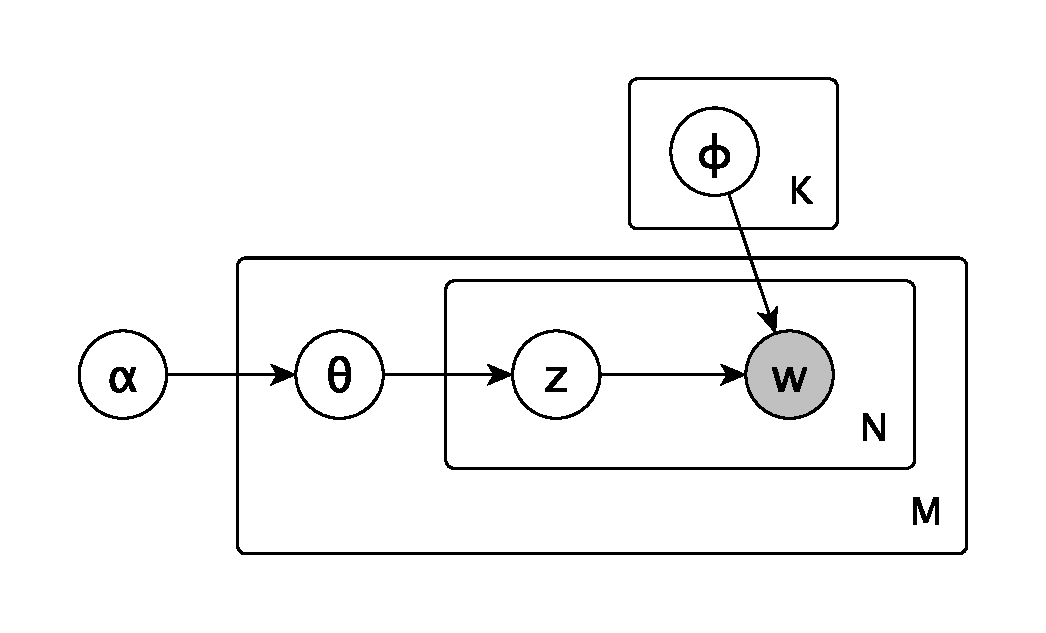
\includegraphics[scale=0.7]{figures/lda-generative-process.eps}
\caption{Diagram of the LDA model.}\label{fig:lda_gen_process}
\end{figure}

The generation of a corpus is done with the following steps~\cite{crain2012dimensionality, blei2003latent}:

\begin{itemize}
    \item \textbf{Draw a distribution over the words for each topic.}
        A sample $\phi_i$ is drawn from a symmetric Dirichlet distribution with parameter $\beta$. 
        This sample represents the distribution of terms for the topic $i$.

        \begin{equation}
            \Phi_i \sim Dir(\beta)
        \end{equation}

        \begin{equation}
            p(\Phi_i | \beta) = \frac{\Gamma(V\beta)}{{\Gamma(\beta)}^V} \prod^V_{v=1}\phi^{\beta-1}_{iv}
        \end{equation}

        Here, $\Gamma$ is the gamma function.

    \item \textbf{Draw a distribution over the topics for each document.}
        A sample $\theta_d$ is drawn from a Dirichlet distribution with parameters $\alpha$.
        This sample represents the distribution of topics for document $d$.

        \begin{equation}
            \Theta_d \sim Dir(\alpha)
        \end{equation}

        \begin{equation}
            p(\Theta_d | \alpha) = \frac{\Gamma(\sum^K_{i=1}\alpha_i)}{\prod_{i=1}^K\Gamma(\alpha_i)}\prod_{i=1}^K\theta_{di}^{\alpha_i-1}
        \end{equation}

    \item For each token with index n:

        \begin{itemize}
            \item \textbf{Draw a topic assignment $z_{dn}$ for the token index $n$.} 
                $z_{dn}$ is drawn from the distribution over topics for each document. 
                That is, $z_{dn}$ is drawn from a multinomial distribution using $\theta_d$ as a parameter.

                \begin{equation}
                    z_{dn} \sim Multinomial(\Theta_d)
                \end{equation}

                \begin{equation}
                    p(z_{dn} = i | \Theta_d) = \theta_{di}
                \end{equation}

            \item \textbf{Draw a token $w_{dn}$.}
                The token $w_{dn}$ is drawn from the topic distribution assigned to the index $n$.
                That is, $w_{dn}$ is drawn from a multinomial with parameter $\phi_{z_{dn}}$.

                \begin{equation}
                    w_{dn} \sim Multinomial(\Phi_{z_{dn}})
                \end{equation}

                \begin{equation}
                    p(w_{dn}=v|z_{dn}=i,\Phi_i) = \phi_{iv}
                \end{equation}

        \end{itemize}

\end{itemize}

The LDA model identifies topics from different terms that occur together.
Consider the case where an LDA model has been used to learn a number of topics.
Two terms that frequently occur together are then likely to be in the same topic.
So, if the same word has been used to express different thoughts, and the word has the same probability in two topics, the words that it co-occurs with can be used to differentiate between the different thoughts.

The task of learning the LDA model is a Bayesian Inference problem.
We have several variables that we cannot observe: the word distribution for the topics ($\phi_i$), the topic assignments for the tokens ($z$), and the topic distribution for the documents ($\theta_d$).
The only observed variables are the words in the document.
We have to approximate the posterior distribution using some sampling method, since it cannot be inferred automatically~\cite{blei2003latent}.

There exist a few algorithms that can be used to learn topics for the LDA model. 
Two of these that has shown to be able to extract useful topics from text are \textit{collapsed Gibbs sampling}~\cite{griffiths2004finding} and \textit{variational Bayes}~\cite{blei2003latent}.  
In collapsed Gibbs sampling, $\theta$ and $\phi$ are marginalized out.
It works by repeatedly sampling the topic assignment $z_{dn}$ for each token, conditioned on the assignments for the other tokens.
Variational Bayes works by using simpler single-variable models to approximate the LDA\@. 
As a consequence, it disregards any dependencies between the variables.
This is the approach used in the original LDA paper~\cite{blei2003latent}.

\subsubsection{Collapsed Gibbs}

% TODO: Write section on collapsed Gibbs
\textit{To be written}

\subsection{Text Clustering}

Cluster analysis is commonly defined as finding groups in a given dataset.
The members of these groups are determined to be similar by a similarity measure~\cite{kaufman2009finding, aggarwal2012survey}.
Since text data is sparse, but yet have a very high dimensionality.
With one dimension per term in the dictionary, it is not uncommon with dimensions in the order of $10^5$.
For this reason, some of the more naive clustering algorithms does not work as well for text data~\cite{aggarwal2012survey}.

In distance-based clustering, a similarity function is used to measure the closeness between two text documents.
For the purpose of measuring the similarity between text objects, the cosine similarity function is most commonly used~\cite{aggarwal2012survey}.
Two different approaches to distance-based clustering are distance-based partitioning, and agglomerative hierarchical clustering.
%For distance-based clustering k-means and k-medoid are two the frequently used algorithms.
%When it comes to text data, k-means is preferred since k-medoid does not work as well for sparse data, and requires more iterations to converge~\cite{aggarwal2012survey}.

\subsubsection{K-means Clustering}

When using the k-means clustering algorithm, the clusters are based upon an initial set of k representatives.
A simple approach to k-means clustering can be seen as:

\begin{enumerate}
    \item Select K seeds from the original dataset
    \item \label{enum:k-means-step-2} Assign the rest of the documents to one of these seeds, based how how similar they are by the similarity function
    \item \label{enum:k-means-step-3} Before each new iteration, select a new centroid for each cluster. This should be the point that is the best central point for the cluster.
    \item Repeat step \ref{enum:k-means-step-2} and \ref{enum:k-means-step-3} until convergence.
\end{enumerate}

A visualization of this can be seen in Figure~\ref{fig:kmeans-iterations}.
One advantage that K-means has over K-medoid is that it requires a small number of iterations, especially compared to K-medoid~\cite{aggarwal2012survey, schutze1997projections}.
However, K-means is rather sensitive to the selection of initial seeds.
One approach is to just select them randomly, or selecting them based on the result of another lightweight clustering method.
A frequently used method is k-means++, that has been shown to improve both the speed and accuracy of k-means clustering~\cite{arthur2007k}.

\begin{figure}[h!]
    \centering
    \thirdsubfig{kmeans-init}{Initial seeds}
    \thirdsubfig{kmeans-iter1}{Iteration 1}
    \newline
    \thirdsubfig{kmeans-init2}{Centroids after iteration 1}
    \thirdsubfig{kmeans-iter2}{Iteration 2}
    \thirdsubfig{kmeans-init3}{Centroids after iteration 2}
    \caption{(a) to (e) shows iterations of K-means until convergence.
        In (e) it can be seen that the new centroids capture the same documents as the previous iteration, and we have converged.}
    \label{fig:kmeans-iterations}
\end{figure}

\subsubsection{Hierarchical Clustering}

% TODO: Write if needed
\textit{To be written if used in the end}

\subsection{Word Embeddings with Word2Vec}

\textit{To be written}

\section{Text Classification}

Text classification is a widely studied field within Computer Science.
It is an important problem in supervised machine learning, and it is the task of assigning one or more classes to a given text document~\cite{aggarwal2012surveyclass}.
The problem is mainly approached with supervised machine learning.
That is, with a dataset that consists of a collection of text documents, where each document has one or more classes assigned to it. % TODO: QUOTE BISHOP
With the help of these labels, a classification model is fitted to the data.
The goal of this is for the model to be able to correctly assign a class to a a previously unseen text document.
Some of these classification models can also produce a probability of a document being of a certain class.
Other models are based on the concept of a margin that separates the classes, and the distance between a data point and a margin can be used to indicate how certain the model is of the assigned label~\cite{tong2001support}.
Example of use cases for text classification is categorization of news articles, document retrieval and email filtering.
There exists several different models for classifying text.
Decision trees, neural networks and Support Vector Machines (SVM) are some have been previously applied to the text domain with successful results~\cite{aggarwal2012survey}.
In this thesis, SVM are the main focus, since they have been studied extensively in the context of active learning. %TODO: CITE ALL OF THE SUPPORT VECTOR MACHINE ACTIVE LEARNING PAPERS

\subsection{Support Vector Machines}

SVMs work by implicitly map the training data to a feature space~\cite{bishop2006pattern}.
The goal is that the data should be linearly separable in the feature space, even if it is not in the input space.
In the case of binary classification, a point is classified by the linear model:

\begin{equation}
    y(x) = w^T \phi(x) + b
\end{equation}

The sign of $y(x)$ determines the label assigned to x.

SVMs work by trying to find the hyperplane that maximizes the margin.
That is, the distance between any point and the decision boundary should be as large as possible.
The hyperplane that gives us the maximum margin can be found by:

\begin{equation}
    \arg\min_{w,b}\frac{1}{2}||w||^2
\end{equation}

In order to allow for better generalization, and for data that isn't completely linearly separable, SVMs make use of slack variables $\xi_n$ to penalize points that are close to the decision boundary~\cite{bishop2006pattern}.
A parameter $C>0$ controls how much effect the slack variables will have.
The equation with the slack variables becomes:

\begin{equation}
    \arg\min_{w,b}\frac{1}{2}||w||^2 + C \sum_n\xi_n.
\end{equation}

A smaller $C$-value allows more points to be misclassified, in order to achieve better generalization.

\subsection{Multi-Label Classification}\label{subsec:multi-label-classification}

Multi-label classification is the type of text classification where one instance can be associated with multiple labels.
It is a generalized version of the multi-class classification problem, where you have more than 2 labels, but each document is only assigned one~\cite{tsoumakas2006multi}.

A common way of solving multi-label classification problems is the Binary Relevance method~\cite{read2011classifier, boutell2004learning}.
It is a way of transforming the multi-label classification problem into several different binary ones.
With Binary Relevance you fit one classification model per label in your data.
Each of these classifiers are then predicting whether or not the document is associated with the corresponding label or not.

\section{Active Learning}

Conventional machine learning systems use a set of available data to find a hypothesis that can explain the patterns.
The purpose of active learning is to allow a system to \textit{select} the data that it wants labeled, and therefore the data it wants to be trained on~\cite{settles2012active}.
An active learning system samples a document to be labeled, and then queries an oracle (often a human annotator) to get the label for that document.
By being able to decide what data to to label and use, the goal is that the system can achieve better results, and that the data will be of higher quality.
A model of the active learning system can be seen in Figure~\ref{fig:active-learning-model}.
The main 

\begin{figure}[!ht]
    \centering
    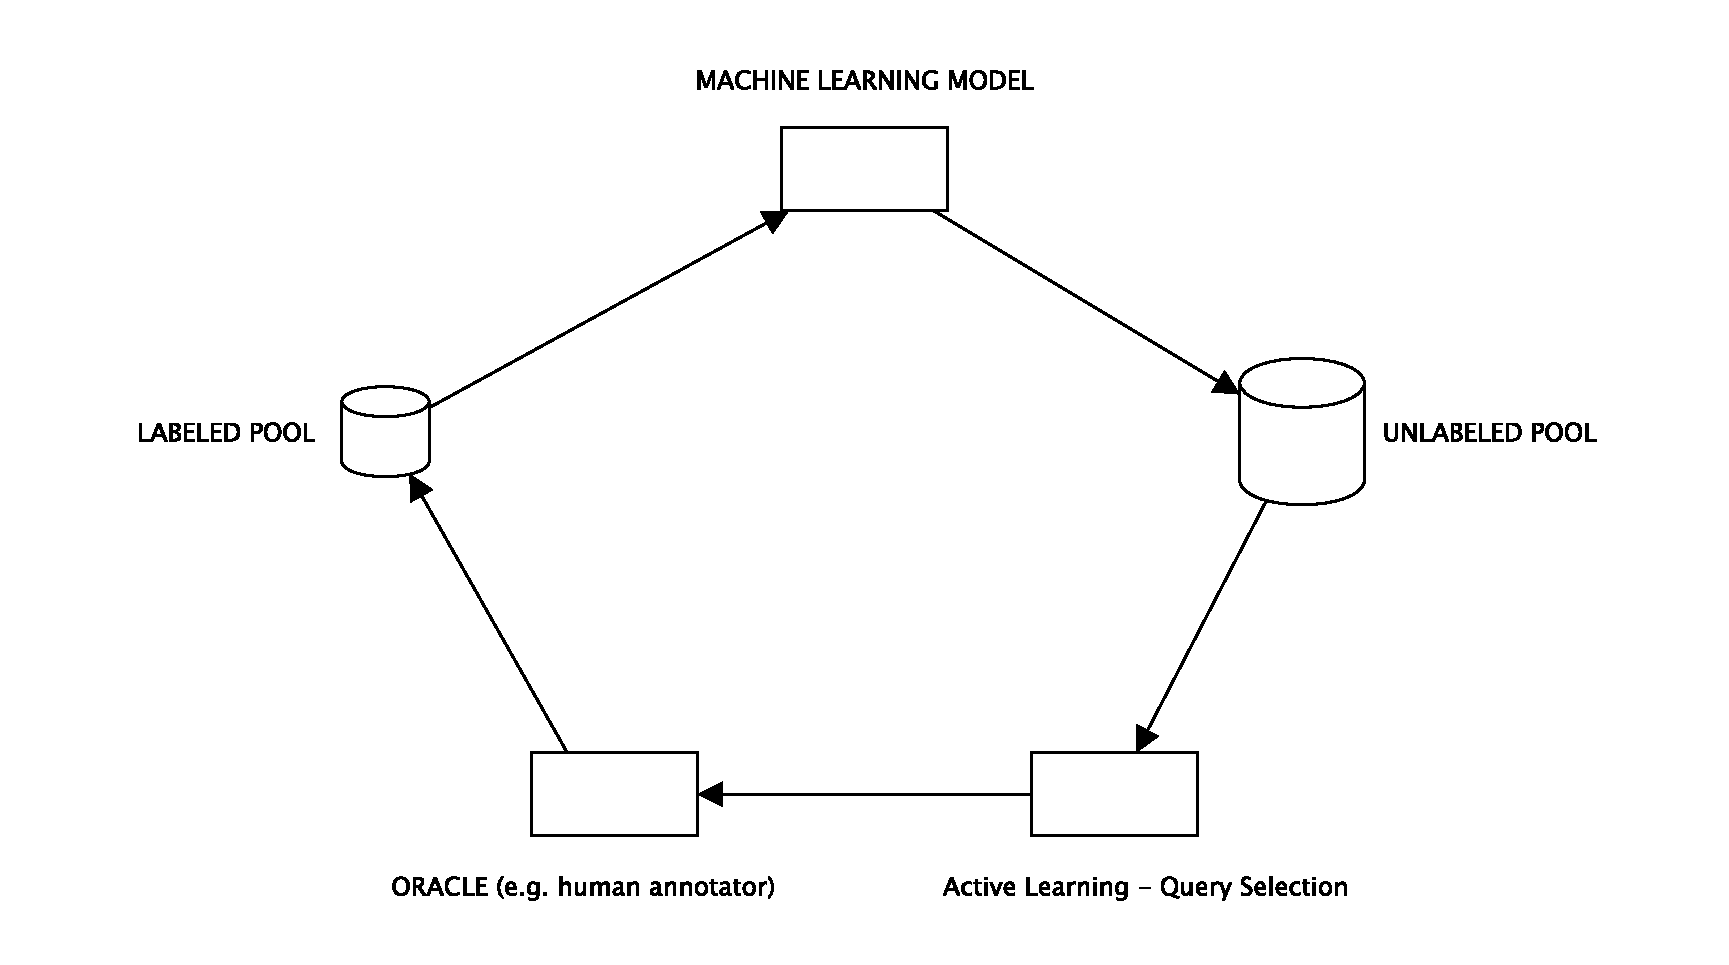
\includegraphics[scale=0.7]{figures/active-learning-model.eps}
    \caption{An overview of an active learning system}
    \label{fig:active-learning-model}
\end{figure}

In several different domains, data is readily available and easy to come by.
But even if the data is abundant, labels for the data is often harder and more expensive to come by~\cite{settles2012active}, especially when it comes to multi-label problems.

The next section will describe different ways to access the documents in active learning systems, followed by some theory of how the samples relate to the hypothesis space.
After that some concrete methods for selecting the samples to queried are described and compared.

\subsection{Pool-Based Sampling}

The main focus is how to select the samples to be labeled.
There are different sampling methods in use, and which one is more appropriate depends on how the data can be accessed.
Pool-based sampling is motivated by the assumption that there exists a large ready pool of data, where only a small portion is labeled~\cite{lewis1994sequential, settles2012active}.
The samples to be labeled is then selecting by evaluating the entire pool of unlabeled data, and select the most appropriate one based on a defined utility measure.
If the entire pool is large, a subset could be used instead.
For applied active learning, pool-based sampling seems to be the most popular choice, but there are some alternatives that have been used in theoretical settings such as stream-based selective sampling.
The difference between stream-based selective sampling and pool-based sampling is the individuality of the decisions in stream-based selective sampling, where you draw one sample at a time from an input source and make the decision whether or not to query a label for it.
For text applications, where a set of data is often readily available, pool-based sampling is often the more appropriate option since you can consider the entire dataset.
Pool-based is therefor the sampling technique that will be considered in this paper.

\subsection{Initial Sampling Selection}

\textit{To be written}

\subsection{Searching the Hypothesis Space}

In machine learning hypothesis is a specific configuration of a model, the purpose of which is to predict outputs on new instances of data by generalizing the training data.
One hypothesis can, for example, be an SVM model with specific values for the parameters.
The set of all possible hypothesis that we are working with the \textit{hypothesis space}.
Following the SVM example, the hypothesis space would be the set of SVM's with the different values that are possible for the parameters.
The hypothesis space is defined as:
% TODO: Big brackets
\begin{equation}
    \begin{aligned}
        \mathcal{H} = \Bigg \{ f | f(x) = \frac{w * \phi(x)}{|w|} \Bigg \}\\
        \text{where~$w \in \mathcal{W}$ and $\mathcal{W}$ is our parameter space}
    \end{aligned}
\end{equation}

The version space the subset of the hypothesis space
The subset of the hypothesis space that in the feature space separates the data is called the version space, which is defined as:

\begin{equation}
    \mathcal{V} = \Bigg \{ f \in \mathcal{H} | y_i f(x_i) > 0 \forall i \in \{i \dots n\} \Bigg \}
\end{equation}

So the version space therefore represents the different hypothesis that make correct predictions on the training data.
Under the assumption that one of the hypothesis can fully separate the data, the version space shrinks when more labeled data is acquired.
So for new labeled instances the hypotheses in the version space will give better predictions for the training data.
Based on this, an active learning algorithm should aim to reduce the size of the version space with each new sample, optimally make it half the size in each iteration.

There exists a useful relationship between the feature space $\mathcal{F}$ and the hypothesis space $\mathcal{H}$ called the \textit{version space duality}~\cite{tong2001support, vapnik1998statistical}.
It states that hyperplanes in the hypothesis corresponds to points in the feature space, and the other way around.
So by selecting points to be labeled, constraints can be enforced on the hypothesis that form the version space.

One approach to this is called that has shown to be successful is \textit{Uncertainty Sampling}~\cite{settles2012active}.
The idea behind SVM is to find a hyperplane that separates two classes in a binary classification with the maximum margin.
Out of the different hyperplanes in the hypothesis space, the version space contains those that can successfully separate the data.
We want to select the points in the feature space that will reduce the amount of the valid hypotheses the most.
Since SVMs tries to find the support vectors that maximizes the decision boundary in the feature space, separating the two classes.
Considering this in $\mathcal{H}$, it will be analogous to the hypothesis in the center of the hypothesis space encompassed constraints set by the labeled points.
What Uncertainty Sampling is predicting the values for the unlabeled points, and then choose the one that it is most uncertain about, the one closest to the decision boundary, to be labeled.
Based on the version space duality, it is a good approximation for dividing the version space in two.

\subsection{Binary Minimization}

Binary Minimization is a generalization of uncertainty sampling, to make it work with multi-label data.
The approach taken is to decompose the multi-label problem to several binary one-vs-rest tasks, like discussed in~\ref{subsec:multi-label-classification}.
The unlabeled point that is chosen for labeling is then the one with the smallest SVM margin across all the binary classification tasks.
By doing this, it does not incorporate the multiple labels into the decision process, but treats all classes individually and equally. 

\subsection{Maximum Loss Reduction with Maximum Confidence}

\subsection{Adaptive Active Learning}

\section{Related Work}

Active learning has been researched in text classification with different approaches.
They can be seen as two categories: searching through the hypothesis space by using the uncertainty of a model, or by exploiting the structure of the data through clustering~\cite{dasgupta2008hierarchical}.

One of the common baselines for active learning is uncertainty sampling~\cite{lewis1994sequential}.
That simply queries the label for the data point the model is most uncertain about.
In~\cite{dasgupta2008hierarchical} hierarchical clustering is used in an active learning system.
The labels are queried from clusters where there is a lot of uncertainty when it comes to the majority label.
By pruning the tree of clusters while querying for labels the goal is to obtain a pruning where each node mostly contains one label.

In \cite{nguyen2004active} they also take advantage of a clustering to select the samples to be labeled in a two-class environment.
They take advantage of that the data points closest to the centroids are the most important ones, and that most data points in one cluster have the same label.
What this approach has in common with a lot of the current research is that it is treating single-label or binary classification problems.
\chapter{Method}
\label{cha:method}

%In this chapter, the method is described in a way which shows how the
%work was actually carried out. The description must be precise and
%well thought through. Consider the scientific term
%replicability. Replicability means that someone reading a scientific
%report should be able to follow the method description and then carry
%out the same study and check whether the results obtained are
%similar. Achieving replicability is not always relevant, but precision
%and clarity is.
%
%Sometimes the work is separated into different parts, e.g.  pre-study,
%implementation and evaluation. In such cases it is recommended that
%the method chapter is structured accordingly with suitable named
%sub-headings.

The task of making a better system for labeling clinical reports was approached with several text mining techniques, support vector machines and a few active learning querying strategies.
At first, the framework and tools used in the system are described, followed by a description of the provided dataset.
Finally, the experiments used to answer the research questions are presented.

\section{Frameworks and Tools}
The entire system was written in Python.
The motivation behind this choice was mainly that, when it comes to machine learning and text mining, most of the existing infrastructure at Sectra is using Python.
This, in combination with the fact that there exists several tools for these purposes in Python, such as \textit{numpy}, \textit{nltk}, \textit{scikit-learn} and \textit{gensim}. %TODO: Find references or links?
All the plotting was done using the \textit{seaborn} and \textit{bokeh} libraries.
\textit{pyLDAvis} was used for some additional visualization purposes with regards to topic models.

However, when it comes to the active learning, there does not seem to be a proven mainstream library that contains a set of readily available algorithms.
In order to achieve better integration between the active learning system and the existing infrastructure at Sectra, as well as making adaptions such as the number of items queried at each iteration, an active learning framework was created.
The ground for this framework were the algorithms presented in Section~\ref{sec:active-learning}.

\section{Datasets}\label{sec:datasets}
In this thesis, two different datasets were used.
The dataset provided by Sectra, as well as Reuters-21578.
The latter was used to be able to simulate a multi-label labeling process, to evaluate how well the different strategies work before being integrated into Sectra's system.
Since the vast majority of the dataset from Sectra was unlabeled, this could not effectively been done using only that.

The set of reports provided by Sectra contained 1068904 different entries, where 493 were initially labeled.
The entries were spread out over several files, stored in the JSON format.
However, those labels were subject to change, so they were mainly used to see if there were any correlation between the labels and clusters during the exploration phase.
A sample report can be seen in Figure~\ref{fig:sample-report}.
The fields include:
\begin{enumerate}
    \item \textbf{ExamId}: The ID of the exam
    \item \textbf{ReportText}: The report written by the physician after the examination
    \item \textbf{Anamnesis}: The patient's account of their medical history
    \item \textbf{PatientAlert}: FILL IN
    \item \textbf{ExamComment}: FILL IN
    \item \textbf{Cancelled}: Whether or not the examination was Cancelled.
    \item \textbf{ExamName}: FILL IN
    \item \textbf{ExamCode}: FILL IN
    \item \textbf{PatientSex}: FILL IN
    \item \textbf{PatientAge}: FILL IN
    \item \textbf{Urgent}: FILL IN
    \item \textbf{Pharma}: FILL IN
\end{enumerate}
%TODO: Include full report
\begin{figure}
\begin{verbatim}
    {
        'ExamId': 24550003, 
        'ReportText': '',
        'Anamnesis': '',
        'Question': '',
        'PatientAlert': ' ', 
        'ExamComment': None, 
        'Canceled': False, 
        'ExamName': '',
        'ExamCode': '81100', 
        'PatientSex': 'MALE', 
        'PatientAge': 71, 
        'Urgent': -1, 
        'Pharma': None
    }
\end{verbatim}
\caption{A sample report from the dataset provided by Sectra}
\label{fig:sample-report}
\end{figure}

The work was mainly concerned with the ReportText field, since it contains the response to the result of the examination.
But the for the complete Active Learning system the Anamnesis was used as well.
The labels that were initially assigned to these reports were:
``Blödning'', ``Infektion'', ``Metabol'', ``Tumör'', ``Cysta'', ``Missbildning'', ``Syndrom'', ``Demens'', ``Hydrocefalus'', ``Infarkt'', ``Kärlsjukdom'', ``Trauma'', ``Systemsjukdom'', ``Inklämmning'' and ``Normal''.

The distribution of labels among these initially labeled reports can be seen in Figure~\ref{fig:class-distribution}
Note that this is only a count of the individual labels, and the multi-label nature of the labeling is not taken into account in the histogram.

\begin{figure}
    \includegraphics[scale=0.5]{figures/class-distribution.png}
    \caption{The distribution over the labels in the initial set of labeled data provided by Sectra}
    \label{fig:class-distribution}
\end{figure}

The Reuters-21578 newswire dataset is widely used when it comes to text classification research, and provides a good multi-label benchmark that can be used to compare how well certain techniques perform to other papers.
All experiments used the \textit{ModApte} split of the dataset, which is commonly used and readily available. %TODO: Footnote with the dataset?
It splits the dataset into a defined set of training and test documents, containing 7.769 and 3.019 entries respectively.
This split contains a subset of the categories, specifically 90 different ones.
Since the clinical dataset from Sectra only contained 15 different categories, this would not mirror that very well, so instead the 15 most common categories of those were taken out.
The distribution of the top 15 Reuters-21578 categories can be seen in Figure~\ref{fig:class-distribution-reuters}.
After filtering out the documents not labeled with any of the top 15 categories, there were 6880 documents left in the training set, and 2646 in the test set.

\begin{figure}
    \includegraphics[scale=0.6]{figures/class-distribution-reuters.png}
    \caption{The distribution over the labels in the Reuters data}
    \label{fig:class-distribution-reuters}
\end{figure}

\section{Pre-Processing and Text Representation}\label{sec:pre-processing}
Before the data was used in the experiments, several pre-processing steps were applied in order to clean the dataset and make it easier to work with.
The steps were:
\begin{enumerate}
    \item First, the fields of interest were extracted.
          In this case that was only the ``ReportText'' field.
    \item White space and punctuation was stripped from the data.
    \item All words were transformed into lowercase.
    \item Filtered out the most common words, as well as very infrequent words.
          Specifically, words occurring less than in 1\% of the documents, as well as words occurring in more than 90\% were removed.
          The idea behind this is that these words would not contribute to differentiating different classes of documents.
          Removing of both frequent and infrequent words is commonly done when working with text and has been done in the context of classification, active learning or topic modelling before~\cite{tong2001support, blei2003latent, brinker2006active, sarioglu2013topic}.
    \item A list of identified common stopwords were removed as well.
          This list of words was based on the Swedish nltk stopwords list.
          After iterating over the dataset seeing the words that frequently occurred this list was extended to incorporate dataset-specific information.
          This included names of the doctors that had written the report.
          By removing names of doctors the idea is to make the system more applicable to new reports, written by other doctors.
    \item Accents from the words were removed.
    \item The text was tokenized and then stemmed using the Porter2 stemmer.
\end{enumerate}
Most of these steps were performed in other reports dealing with text analysis in the form of classification or active learning~\cite{tong2001support, blei2003latent, brinker2006active, sarioglu2013topic}.

After transforming the text into a sequence of tokens, the final step before using it with the models was to create a representation that would be beneficial for them to work on.
The representation chosen is a matrix of tokens count, so each document is represented by the counts of each token, disregarding the order of the tokens.
In order to get some positional information into the representation additional tokens are stored, besides the standalone tokens processed as described above.
The additional tokens are bigrams.
Bigrams are pairs of tokens (i.e. processed words), so the frequency of how often such a pair occurs in the document is stored alongside the regular one word tokens.

\section{Exploratory Study}\label{sec:exploratory-study}
For the exploratory study we used the representation described in Section~\ref{sec:pre-processing}, but without the bigrams.
The main goal of this phase was to get to know and to better understand the dataset.
A part of this goal was to go through the fields for the different reports to see how they worked and what values could be expected.
Another big part of this was to visualize the dataset in different ways.
In order to visualize the data in a 2D plot, t-distributed stochastic neighbor embedding (t-SNE) was used.
It is a dimensionality reduction technique, that is able to transform high dimensional data into two dimensions, trying to retain as much variance as possible.

The first step was to fit an LDA model to the data.
For the purpose of exploring the data, the number of topics were chosen to be a 100, with the hope of it not resulting in too granular topics that would be hard to manually analyze. %TODO: How many topics did other reports include?
In order to being able to visualize the data in a meaningful way, a subset of X reports were used to begin with.
The data points were plotted in a 2D plot after reducing the dimensions using t-SNE.
Since each data point is associated with several different topics, there exists several way of coloring each data point in order to gain an understanding of them.
In this case, simply the topic with the highest probability for a given data point was used to determine the color.
A plot of this can be seen in Figure~\ref{fig:lda-dist}.
Although it might be hard to interpret as a 2D plot in this report, using the \textit{bookeh} library an interactive plot was generated, so hovering over each data point would show the content of the report, making this a convenient way to explore the data and the generated topics.

\begin{figure}
    \centering
    \includegraphics[scale=0.25]{figures/lda-2d-distribution.png}
    \caption{A 2D plot of the text data, where each point is colored by the most prominent topic}
    \label{fig:lda-dist}
\end{figure}

Samples of the generated topics can be seen in [FIGURE].
Another way to visualize the topics for inspection is using the techniques described by Sievert et al\@.~\cite{sievert2014ldavis}.
They propose a \textit{relevance} measure where the probability for a certain term within a topic is weighted against how common that topic is in the entire corpus.
The interactive interface provided by \textit{pyLDAvis} can be seen in Figure~\ref{fig:ldavis-sample}.

A word2vec model was used on the entire dataset to evaluate see the relationship between terms and find possible synonyms.
In order to find synonyms, all words in the dataset that had a similarity over 95\% were manually inspected.
This model was in addition to this used to identify names and other identifiers in the reports, as they would come up as similar entities from the model.
Accomplishing this was done by exploring the data through an interactive plot, after using t-SNE to reduce the number of dimensions.

\begin{figure}
    \centering
    \includegraphics[scale=0.3]{figures/ldavis-sample.png}
    \caption{A way to visualize and analyze topics based on their relevance and frequency}
    \label{fig:ldavis-sample}
\end{figure}

\section{Experiments to Answer the Research Questions}
In this section the experiments used to answer the research questions are described.
There is one experiment designed for each questions, and the second one is of a more literature study.
The first experiment is trying to identify reports that are deemed to be invalid, the second one is a study to see what are the alternatives to labeling data points at random, and the third is to evaluate which one of the alternatives is the best.

\subsection{Filter Out Invalid Clinical Reports Using Topic Models and Clustering}

Here, the task was to evaluate how well topic modeling and clustering could be used to filter out invalid reports.
Invalid reports are here considered to be reports that describe a situation where an examination never took place.
This can be because of a deceased patient, a patient being moved to another hospital, a patient did not show up or simply did not want to go through with the examination for any reason.

Different topic model and cluster sizes were tested for this purpose.
The topic model used was Latent Dirichlet Allocation, and the clustering algorithm used was K-means.
The K-means clustering used the latent topic vectors produced by the topic model as representation when finding the clusters.
As described in Section~\ref{sec:topic-modeling}, in order to use the LDA model the number of topics has to be selected.
The same applies to K-means, which is described in Section~\ref{sec:k-means}.
Selecting the best model was done by evaluating different number of topics $k_{LDA}$ and the number of clusters $k_{c}$.
The topic models were evaluated with $k_{LDA}$ set to 25, 50, 75, 100, 150, 200.
Evaluating the clusters were done by combining the different topic models with the different cluster sizes to find the best combination.
The different combinations can be seen in Table~\ref{tab:topic-kmeans-configs}.
\begin{table}[!ht]
    \centering
    \begin{tabular}{|ccc|}
        \hline
        ID & $k_{LDA}$ & $k_{c}$\\
        \hline
        1 & 25 & 25 \\
        2 & 25 & 50 \\
        3 & 25 & 75 \\
        4 & 25 & 100 \\
        5 & 25 & 150 \\
        6 & 25 & 200 \\
        7 & 50 & 25 \\
        8 & 50 & 50 \\
        9 & 50 & 75 \\
        10 & 50 & 100 \\
        11 & 50 & 150 \\
        12 & 50 & 200 \\
        13 & 75 & 25 \\
        14 & 75 & 50 \\
        15 & 75 & 75 \\
        16 & 75 & 100 \\
        17 & 75 & 150 \\
        18 & 75 & 200 \\
        \hline
    \end{tabular}
    \quad
    \begin{tabular}{|ccc|}
        \hline
        ID & $k_{LDA}$ & $k_{c}$\\
        \hline
        19 & 100 & 25 \\
        20 & 100 & 50 \\
        21 & 100 & 75 \\
        22 & 100 & 100 \\
        23 & 100 & 150 \\
        24 & 100 & 200 \\
        25 & 150 & 25 \\
        26 & 150 & 50 \\
        27 & 150 & 75 \\
        28 & 150 & 100 \\
        29 & 150 & 150 \\
        30 & 150 & 200 \\
        31 & 200 & 25 \\
        32 & 200 & 50 \\
        33 & 200 & 75 \\
        34 & 200 & 100 \\
        35 & 200 & 150 \\
        36 & 200 & 200 \\
        \hline
    \end{tabular}
    \caption{The different combination of topic model/k-means clusters that were evaluated.}
    \label{tab:topic-kmeans-configs}
\end{table}

In order to evaluate how well they performed on the clinical data, a set of reports had to be marked as valid/invalid.
This was done by creating a script that presented a report to the user, and allowed it to be marked as valid or invalid.
At first X reports were labeled.
After this set, the labels were skewed, containing only Y invalid reports, which makes up Y/X\% of the labels.
In order to get a more balanced dataset, $X_2$ of the valid reports were dismissed at random.

80 000 reports were used in the experiment, and they were selected at random.
The reason for only using a subset is that the number of reports available would be too big to use in the final active-learning system. %TODO: Refer
The models were fitted on 72 000, or 90\%, of these reports, and the additional 10\% were used as a held-out set to evaluate the models.
To determine which topic model and clustering technique that should be used in the filtering of invalid reports, their perplexity was compared and the models with the best perplexity was chosen.
Perplexity is used in the original LDA paper by Blei et al\@.~\cite{blei2003latent} to compare different number of topics.

In order to make the models able to separate the invalid reports from the valid reports, they had to be manually analyzed, since they were not fitted for this specific purpose (they are both unsupervised techniques).
Approaching this in a way that would result in the models overfitted to the analyzed data could be hard since they are manually analyzed. 
To get an evaluation that was not as biased, the labeled reports were split into a training set to be analyzed and a validation set, containing 80\% and 20\% of the reports, respectively.

First, the LDA model was analyzed.
This was done by inspecting the topics in the same way that was done in the exploratory study, Section~\ref{sec:exploratory-study}.
Based on the distribution of the most likely topics for the invalid reports in the traning set, topics with a high indication of a report being invalid was selected for further analysis.
A combination these topics together with the length of the report text, as well as the number of topics assigned with a high probability to a report were used to determine whether or not a report was invalid or not.

Filtering out these reports with K-means results in a simpler method.
K-means does not give any probability for its clusters, so filtering by the clusters must be done as a binary decision.

\subsection{Alternatives to Label Reports at Random}\label{sec:exp1-method}

This was done mainly by doing a literature study and exploring the relation between the initial set of labeled data with the structure of the data through clustering and topic analysis.
At first, the labeled data was transformed using the LDA and k-means models.
After that, they were plotting in the same 2D space as before.
The color of the labeled data was set based on the first label, after an instance's labels had been sorted.

Just as before this was an interactive plot, hovering over the data points revealed the report as well as the topics and the cluster assigned to the data point.
The goal of this was to see if there existed a relationship between the topics/clusters and the labeled assigned to the data point.
Based on multi-label nature of the data and the results of this plot, active learning approaches were researched, with the goal of identifying methods that would be applicable in a multi-label setting.
The research touched upon both methods that exploit the structure of the data, and methods that are purely uncertainty based.

\subsection{How Well Does the Alternatives Work?}

After establishing the techniques that had some indication on providing a better labeling process than sampling documents at random, they were evaluated.
In order to provide a thorough evaluation of how well they techniques perform a set of already labeled reports were needed.
For this reason, the Reuters-21578 dataset was used.
The properties of the dataset, as well as a comparison between it and the clinical data provided by Sectra can be found in Section~\ref{sec:datasets}.
The dataset is common in active learning research and has been used by Brinker et al\@.~\cite{brinker2006active} and Yang et al\@.~\cite{yang2009effective}, among others.
With this set of of labeled reports, a simulation could be used to compare the different strategies with different metrics.
The metrics used were:
\begin{enumerate}
    \item Accuracy
    \item Micro recall
    \item Macro recall
    \item Micro precision
    \item Macro precision
    \item Micro F1-Score
    \item Macro F1-Score
\end{enumerate}

These are described in Section~\ref{sec:evaluation-metrics} and are frequently used to compare different active learning methods, for example by Yang et al\@.~\cite{yang2009effective}, Dasgupta et al\@.~\cite{dasgupta2008hierarchical} and Li et al\@.~\cite{li2013active}, among others.
In addition to these metrics, the time it took to query samples with each model was also compared, and the how the distribution looked at the different stages.
This is because the doctors wanted a more uniform distribution over labels on the labeled samples, i.e. a smaller ratio between the most common label and the least common one.

With this dataset, the same pre-processing steps that were applied to the clinical dataset were applied to the Reuters data too.
Some modifications of this includes the stopwords, instead of a curated list of words, the unmodified list of english stopwords provided by \textit{nltk} was used.
The main goal was to compare how the different techniques affected the labeled dataset, and how well an SVM model performed on it.
Optimizing the process for the particular model and dataset was therefore not the goal, but instead offering a more comprehensive comparison.

The strategies compared were: 
\begin{itemize}
    \item \textit{Binary Version Space Minimization}: Described in Section~\ref{subsec:binmin}
    \item \textit{Maximum Loss Reduction with Maximum Confidence}: Described in Section~\ref{subsec:mmc}
    \item \textit{Adaptive Active Learning}: Described in Section~\ref{subsec:adaptive-active-learning}
\end{itemize}

When it comes to the initial samples that needs to be labeled in order for the strategies to base their selection on something.
This sample were evaluated both by selecting it at random, and selecting then by sampling from the clusters.
Sampling from the clusters was done by iterating over the clusters and selecting an equal number of data points from the clusters, at random.
The clustering configuration was the one chosen in Section~\ref{sec:exp1-method}.

Since the different models may depend on the initial samples in different ways, different initial sizes were evaluated.
This is also done by Yang et al\@.~\cite{yang2009effective}.
In their paper they tried quite large initial sample sizes.
Here, the sizes evaluated are: 10, 50, 100, 200.
The reason for this is that an large initial sample size would make it hard for the human annotator to see a difference in the class balance early on.
The different active learning configurations that were tried is displayed in Table~\ref{fig:active-learning-configurations}
In total there were 18 configurations, based upon the three different methods.

\begin{table}
    \begin{tabular}{|cccc|}
        \hline
        \textbf{ID} & \textbf{Active Learning Strategy} & \textbf{Initial Sampling} & \textbf{Initial Sample Size}\\
        \hline
        1 & Binary Version Space Minimization & Random & 10\\
        2 & Binary Version Space Minimization & Random & 50\\
        3 & Binary Version Space Minimization & Random & 100\\
        4 & Binary Version Space Minimization & Random & 200\\
        5 & Binary Version Space Minimization & Sampled from clusters & 10\\
        6 & Binary Version Space Minimization & Sampled from clusters & 50\\
        7 & Binary Version Space Minimization & Sampled from clusters & 100\\
        8 & Binary Version Space Minimization & Sampled from clusters & 200\\
        9 & Maximum Loss Reduction with Maximum Confidence & Random & 10\\
        10 & Maximum Loss Reduction with Maximum Confidence & Random & 50\\
        11 & Maximum Loss Reduction with Maximum Confidence & Random & 100\\
        12 & Maximum Loss Reduction with Maximum Confidence & Random & 200\\
        13 & Maximum Loss Reduction with Maximum Confidence & Sampled from clusters & 10\\
        14 & Maximum Loss Reduction with Maximum Confidence & Sampled from clusters & 50\\
        15 & Maximum Loss Reduction with Maximum Confidence & Sampled from clusters & 100\\
        16 & Maximum Loss Reduction with Maximum Confidence & Sampled from clusters & 200\\
        17 & Adaptive Active Learning & Random & 10\\
        18 & Adaptive Active Learning & Random & 50\\
        19 & Adaptive Active Learning & Random & 100\\
        20 & Adaptive Active Learning & Random & 200\\
        21 & Adaptive Active Learning & Sampled from clusters & 10\\
        22 & Adaptive Active Learning & Sampled from clusters & 50\\
        23 & Adaptive Active Learning & Sampled from clusters & 100\\
        24 & Adaptive Active Learning & Sampled from clusters & 200\\
        \hline
    \end{tabular}
    \caption{The different configurations of active learning strategies evaluated}
    \label{fig:active-learning-configurations}
\end{table}

\chapter{Results}
\label{cha:results}

%This chapter presents the results. Note that the results are presented
%factually, striving for objectivity as far as possible.  The results
%shall not be analyzed, discussed or evaluated.  This is left for the
%discussion chapter.

%In case the method chapter has been divided into subheadings such as
%pre-study, implementation and evaluation, the result chapter should
%have the same sub-headings. This gives a clear structure and makes the
%chapter easier to write.

%In case results are presented from a process (e.g. an implementation
%process), the main decisions made during the process must be clearly
%presented and justified. Normally, alternative attempts, etc, have
%already been described in the theory chapter, making it possible to
%refer to it as part of the justification.

In this chapter the results are described.
First, the outcome from the exploratory study is presented, followed by the different experiments.
The first experiment, filtering out invalid reports, presents the evaluation of the topic model used to filter out the reports, as well as the specific topics and how they were used in the process.
In the second one, the methods considered and the decisions behind which ones that were appropriate are presented.
Finally, the last section goes through the result of evaluating the different active learning techniques.

\section{Exploratory Study}


\section{Filter Out Invalid Clinical Reports Using Topic Models and Clustering}\label{sec:exp1-result}


Based on these findings, reports were determined to be invalid or not based on if they fulfilled both of the following criteria:
\begin{itemize}
    \item Having either topic 1 or 17 as its most probable topic.
    \item Not having more than 6 prominent topics assigned to it.
\end{itemize}

The evaluation on the validation set can be seen in Table~\ref{tab:exp1-eval}.
In the figure you can also see the results of the logistic regression classifier, which was fitted with the topic vectors as features and the invalid/valid labels as targets.

\begin{table}[h!]
    \centering
    \begin{tabular}{|c|cc|}
        \hline
        & \textbf{Manual Identification} & \textbf{Logistic Regression} \\
        \hline
        \textbf{Precision} & 97.2\% & 98.7\% \\
        \textbf{Recall} & 100\% & 100\% \\
        \textbf{$F_1$-measure} & 98.6\% & 99.4\%\\
        \textbf{Accuracy} & 97.9\% & 99.1\%\\
        \hline
    \end{tabular}
    \caption{The results of the classification of the invalid reports. The manual identification column represents the use of manual interpretation of the LDA topics to find the invalid reports.}
    \label{tab:exp1-eval}
\end{table}

A comparison of how long time it took for the different strategies can be seen in Figure~\ref{fig:al-time-dist}.

\begin{figure}[!ht]
    \centering
    \includegraphics[width=\textwidth]{figures/time-distribution.png}
    \caption{The percentage of time used on the different strategies during one iteration.}
    \label{fig:al-time-dist}
\end{figure}

\section{Alternatives to Labeling at Random}



Based on the knowledge that there exists a pattern, the initial goal was to find some methods that could exploit this.
Some active learning approaches using different forms of clustering, such as Dasgupta et al\@'s approach using hierarchical clustering~\cite{dasgupta2008hierarchical}, would be good contenders.
However, the method described by Dasgupta et al\@. is made for the single-label case with no obvious way of extending the technique into multi-label.
The same applies to the density based technique suggested by Attenberg et al\@.~\cite{attenberg2013class}.

Most of the active learning research seems to be focused on binary, and maybe multi-class classification.
Thus the methods described in Section~\ref{sec:active-learning} where the ones decided on.
Methods that are fully reliant on a models certainty, such as Binary Version Space Minimization (BSVM)~\cite{brinker2006active} are used.
Furthermore, methods incorporating some information about the data in the form of label cardinality is included as well.
These techniques are Maximum Loss Reduction with Maximum Confidence (MMC) and Adaptive Active Learning (AAL)~\cite{yang2009effective, li2013active}.
An attempt to take advantage of the structure of the data is done by selecting the initial samples from different clusters, as described in Section~\ref{sec:exp2-method}.

The plot for evaluating accuracy on the strategies with initial sample sizes of 25, 50 and 100 can be seen in Figure~\ref{fig:al-accuracy-25}, Figure~\ref{fig:al-accuracy-50}, and Figure~\ref{fig:al-accuracy-100} respectively.
Note that when retrieving the initial sample from the clusters, only samples with label cardinality 1 was retrieved after 10 tries.
MMC requires at least two different label cardinalities in the initial sample in order for the logistic regression model to work.
For that reason, MMC with cluster initialization was not evaluated.
In Table~\ref{tab:active-learning-accuracy-25} to Table~\ref{tab:active-learning-accuracy-100} it can be seen how many labels were required to reach a certain accuracy.

\includeaccuracyplot{25}
\includeaccuracyplot{50}
\includeaccuracyplot{100}

\begin{table}
    \centering
    \begin{tabular}{|cccccccc|}
        \hline
        \textbf{Strategy} & \textbf{Initial Sample} & \textbf{75 \%} & \textbf{80 \%} & \textbf{85 \%} & \textbf{87 \%} & \textbf{88 \%} & \textbf{89 \%}\\
        \hline
        BSVM & Random & 475 & 650 & 1100 & 1450 & 1675 & 2425\\
        BSVM & Cluster & 425 & 650 & 1100 & 1575 & 1700 & 2425\\
        MMC & Random & 600 & 775 & 1050 & 1250 & 1575 & N/A\\
        MMC & Cluster & N/A & N/A & N/A & N/A & N/A & N/A\\
        Adaptive & Random & 400 & 575 & 975 & 2425 & N/A & N/A\\
        Adaptive & Cluster & 375 & 550 & 1025 & 2300 & N/A & N/A\\
        Random & Random & 550 & 900 & 1700 & N/A & N/A & N/A\\
        \hline
    \end{tabular}
    \caption{The number of labeled reports in total that the strategies required to achieve the different accuracy values, with initial sample size 25. Only results for the first 2500 data points that were labeled are considered.}
    \label{tab:active-learning-accuracy-25}
\end{table}

\begin{table}
    \centering
    \begin{tabular}{|cccccccc|}
        \hline
        \textbf{Strategy} & \textbf{Initial Sample} & \textbf{75 \%} & \textbf{80 \%} & \textbf{85 \%} & \textbf{87 \%} & \textbf{88 \%} & \textbf{89 \%}\\
        \hline
        BSVM & Random & 450 & 625 & 1075 & 1550 & 1750 & N/A\\
        BSVM & Cluster & 450 & 675 & 1125 & 1600 & 1725 & 2450\\
        MMC & Random & 625 & 775 & 1100 & 1325 & 1675 & N/A\\
        MMC & Cluster & N/A & N/A & N/A & N/A & N/A & N/A\\
        AAL & Random & 375 & 575 & 925 & N/A & N/A & N/A\\
        AAL & Cluster & 425 & 575 & 1075 & N/A & N/A & N/A\\
        Random & Random & 550 & 775 & 1575 & N/A & N/A & N/A\\
        \hline
    \end{tabular}
    \caption{The number of labeled reports in total that the strategies required to achieve the different accuracy values, with initial sample size 50. Only results for the first 2500 data points that were labeled are considered.}
    \label{tab:active-learning-accuracy-50}
\end{table}

\begin{table}
    \centering
    \begin{tabular}{|cccccccc|}
        \hline
        \textbf{Strategy} & \textbf{Initial Sample} & \textbf{75 \%} & \textbf{80 \%} & \textbf{85 \%} & \textbf{87 \%} & \textbf{88 \%} & \textbf{89 \%}\\
        \hline
        BSVM & Random & 400 & 600 & 1125 & 1525 & 1775 & N/A\\
        BSVM & Cluster & 450 & 675 & 1125 & 1600 & 1725 & 2450\\
        MMC & Random & 600 & 750 & 1100 & 1325 & 1675 & N/A\\
        MMC & Cluster & N/A & N/A & N/A & N/A & N/A & N/A\\
        AAL & Random & 350 & 525 & 925 & 2450 & N/A & N/A\\
        AAL & Cluster & 450 & 600 & 1025 & N/A & N/A & N/A\\
        Random & Random & 475 & 775 & 1700 & N/A & N/A & N/A\\
        \hline
    \end{tabular}
    \caption{The number of labeled reports in total that the strategies required to achieve the different accuracy values, with initial sample size 100. Only results for the first 2500 data points that were labeled are considered.}
    \label{tab:active-learning-accuracy-100}
\end{table}

The micro and macro $F_1$-score, recall and precision for the initial sample size of 25 can be seen in Figure~\ref{fig:result-25}.
The same evaluation for the initial sample size of 50 and 100 can be seen in Figure~\ref{fig:result-50} and Figure~\ref{fig:result-100}, respectively.

\includeevaluationplot{25}
\includeevaluationplot{50}
\includeevaluationplot{100}

\section{Evaluating the Label Balance}

The last part to evaluate is how the different Active Learning techniques effected the balance of the labels.
For the Reuters dataset, how the overall distribution of the labels is can be seen in Figure~\ref{fig:class-distribution-reuters}.
After random sampling, the distribution can be seen in Figure~\ref{fig:class-distribution-reuters-random}.
For comparison with the techniques it shows the labels both after 500 labels are added, and 2000.
In order to be able to compare it with the other techniques easily, the plot contains the distribution after both 500 and 2000 labels are acquired.
The distribution after sampling with the original BSVM can be seen in Figure~\ref{fig:class-distribution-reuters-binmin}, and with the initial samples taken from clusters in Figure~\ref{fig:class-distribution-reuters-binmin-clusters}.
For MMC the distribution can be seen in Figure~\ref{fig:class-distribution-reuters-mmc}.
The corresponding plots for Adaptive Active Learning can be seen in Figure~\ref{fig:class-distribution-reuters-adaptive} and Figure~\ref{fig:class-distribution-reuters-adaptive-clusters}.

\begin{figure}
    \centering
    \thirdsubfigimg{distribution-RandomSampling-25-500}{The class distribution from random sampling after 500 labels}
    \thirdsubfigimg{distribution-RandomSampling-25-2000}{The class distribution from random sampling after 2000 labels}
    \caption{The distribution of labels after random sampling}
    \label{fig:class-distribution-reuters-random}
\end{figure}

\begin{figure}
    \centering
    \thirdsubfigimg{distribution-BinaryMinimization-25-500}{The class distribution from BSVM after 500 labels}
    \thirdsubfigimg{distribution-BinaryMinimization-25-2000}{The class distribution from BSVM after 2000 labels}
    \caption{The distribution of labels after BSVM}
    \label{fig:class-distribution-reuters-binmin}
\end{figure}


\begin{figure}
    \centering
    \thirdsubfigimg{distribution-ClusterBinaryMinimization-25-500}{The class distribution from BSVM, with the initial sample from clusters, after 500 labels}
    \thirdsubfigimg{distribution-ClusterBinaryMinimization-25-2000}{The class distribution from BSVM, with the initial sample from clusters, after 2000 labels}
    \caption{The distribution of labels after BSVM with clustering}
    \label{fig:class-distribution-reuters-binmin-clusters}
\end{figure}

\begin{figure}
    \centering
    \thirdsubfigimg{distribution-MMC-25-500}{The class distribution from MMC after 500 labels}
    \thirdsubfigimg{distribution-MMC-25-2000}{The class distribution from MMC after 2000 labels}
    \caption{The distribution of labels after MMC}
    \label{fig:class-distribution-reuters-mmc}
\end{figure}

\begin{figure}
    \centering
    \thirdsubfigimg{distribution-AdaptiveLearner-25-500}{The class distribution from Adaptive Active Learning after 500 labels}
    \thirdsubfigimg{distribution-AdaptiveLearner-25-2000}{The class distribution from Adaptive Active Learning after 2000 labels}
    \caption{The distribution of labels after Adaptive Active Learning}
    \label{fig:class-distribution-reuters-adaptive}
\end{figure}

\begin{figure}
    \centering
    \thirdsubfigimg{distribution-ClusterAdaptiveLearner-25-500}{The class distribution from Adaptive Active Learning, with the initial sample from clusters, after 500 labels}
    \thirdsubfigimg{distribution-ClusterAdaptiveLearner-25-2000}{The class distribution from Adaptive Active Learning, with the initial sample from clusters, after 2000 labels}
    \caption{The distribution of labels after Adaptive Active Learning with clustering}
    \label{fig:class-distribution-reuters-adaptive-clusters}
\end{figure}

In Table~\ref{tab:distribution-result-500} the results of the evaluation after 500 new labels can be seen.
The corresponding table for the evaluation after 2000 new labels can be seen in Table~\ref{tab:distribution-result-2000}.

\begin{table}[h!]
    \centering
    \begin{tabular}{|ccccc|}
        \hline
        \textbf{Strategy} & \textbf{Initial Sample} & \textbf{Top Class} & \textbf{Top 3 Classes} & \textbf{Small/Big Ratio}\\
        \hline
        Random & Random &  34.9 \% & 65.5 \% & 32.0 \\
        BSVM & Random &  22.0 \% & 49.8 \% & 45.0 \\
        BSVM & Clusters & 19.8 \% & 49.0 \% & 80.0 \\
        Adaptive & Random & 14.8 \% & 38.5 \% & 5.4 \\
        Adaptive & Clusters & 14.5 \% & 38.2 \% & 6.65 \\
        MMC & Random & 13.1 \% & 35.2 \% & 8.2 \\
        \hline
    \end{tabular}
    \caption{The results after analyzing the label distribution after 500 new labels has been added.}
    \label{tab:distribution-result-500}
\end{table}

\begin{table}[h!]
    \centering
    \begin{tabular}{|ccccc|}
        \hline
        \textbf{Strategy} & \textbf{Initial Sample} & \textbf{Top Class} & \textbf{Top 3 Classes} & \textbf{Small/Big Ratio}\\
        \hline
        Random & Random & 36.65 \% & 64.6 \% & 29.4 \\
        BSVM & Random & 16.0 \% & 42.4 \% & 7.5 \\
        BSVM & Clusters & 15.7 \% & 41.5 \% & 7.3 \\
        Adaptive & Random & 36.4 \% & 56.2 \% & 43.4 \\
        Adaptive & Clusters & 34.5 \% & 54.8 \% & 41.0 \\
        MMC & Random & 16.7 \% & 41.2 \% & 9.3 \\
        \hline
    \end{tabular}
    \caption{The results after analyzing the label distribution after 2000 labels has been added.}
    \label{tab:distribution-result-2000}
\end{table}
\chapter{Discussion}
\label{cha:discussion}

The discussion chapter is separated into three parts.
First, it goes through and analyzes the results from the experiments in Chapter~\ref{cha:experiments}.
This is followed by an analysis of the methods used to conduct those experiments.
The related works 
At last the work is discussed in a wider context, based on the ethical and societal impact techniques like these may have.

\section{Results}
\label{sec:discussion-results}

Here the results are analyzed and discussed for the different experiments in Chapter~\ref{cha:experiments}.
They are discussed based on their relation to the research questions.

\subsection{Experiment 1}

The first experiment was conducted to be able to answer the first research question, which treated how well the SVM model perform on the data labeled by the active learning process.
Looking at how the different strategies perform in terms of accuracy and $F_1$-score, it is clear that for the first 600-700 labels, Maximum Loss Reduction with Maximum Confidence (MMC) performs considerably worse than the rest.
That is including random sampling.
It is equally clear that it performs better when the initial sample is bigger.
One reason behind this may be MMC's dependence on the label cardinality of the samples.
MMC's dependence on label cardinality can be seen in Section~\ref{subsec:mmc}.
If the information on label cardinality is not varied, the predictions that MMC base its calculations upon will not be as good.
In the paper by Yang et al\@.~\cite{yang2009effective}, MMC performs significantly better than than Binary Version Space Minimization (BSVM) at all stages.
One obvious reason for this discrepancy could be the implementation used in this paper, as is discussed in Section~\ref{sec:discussion-results}.
Another one can be the initial sample sizes used in their paper, even when they compare different initial sample sizes, they start at 100 samples and go up to a 1000.

Adaptive Active Learning (AAL) performs the best of the evaluated strategies in both accuracy and $F_1$-score, when only a few hundred samples has been labeled. 
A probable reason for this is the extra computations the strategy does in order to find the best weight between the certainty based, and the cardinality based, strategies.
If the cardinality predictions is not deemed to be very good in the beginning, it would simply put more weight on the certainty measure, and vice versa.

BSVM on the other hand performs very similarly to random sampling for the first samples.
The reason for this is rather simple.
The strategy finds the class that is the closest to the decision boundary for each data point, and selects the minimum distance of those.
If there are several documents with the same minimum value they are selected at random from those.
Until all classes has been sampled at least one, the minimum for all data points will be the same class, and it will be equal among all data points.
Therefore, it will be the same as selecting randomly among all the samples.
However, when all classes have been sampled, and quickly outperforms the random sampling in terms of accuracy and $F_1$-score.

In the end, the different strategies all perform better than random sampling.
The ones that are based on MMC and BSVM tend to perform a bit better than AAL when more than 1200-1300 samples are added.
This may very well be related to the fact that the distributions for MMC and BSVM is considerably more uniform when a lot of labels have been requested.
BSVM is the only technique that reached 89 \% accuracy within the first 2500 labels to be labeled.
It is possible that other techniques would have reached it given more labels, but it is clear that BSVM reaches a peek accuracy earlier.
The technique always tries to sample from the most uncertain category.
The lack of reports in this category can be the thing that prohibits the other strategies from achieving a higher accuracy.

The initial clustering of reports did not seem to make as much of a difference as the strategy used.
This makes sense, the initial sample size only makes up for a little bit of the overall set of labeled reports.
Worth noting is that the SVM model performs worse for the first couple of iterations with initial clustering.
It quickly recovers after this and seems to perform as well, or slightly better, compared to the randomly initialized counterpart.
The reason for the low initial performance might be due to skewed dataset.
If we assume that the clusters captures a bit of the label information, then the labels should be more evenly distributed in the initial sample.
On the other hand, if the test set contains mostly one or two labels, the initial set will not have seen as much of these and will therefore not be as accurate in predicting them.
This would then greatly reduce the evaluation.

All clusters will not have the same number of members.
If most of the documents with a high label cardinality got assigned the same populous cluster, they might get neglected from the initial sample since an equal number of reports was taken from each cluster.
This could be a reason for the clustering approach to initial sampling only obtained samples with label cardinality 1, and therefore excluding MMC from the process.

\subsection{Experiment 2}

In order to satisfy the request of a more labeled dataset, which is of concern in the second research question, the distribution of labels were analyzed.
Looking at this distribution it is instantly clear that the three strategies outperforms random sampling significantly.
MMC and AAL are by far the most balanced one after only 500 labels are labeled.
When 2000 data points are labeled, BSVM is the most balanced one, albeit slightly compared to MMC.
It can probably be attributed to it selecting the most uncertain class in every iteration.
The most uncertain class is probably the one with the fewest samples, causing the distribution to be more uniform over time.

While BSVM always selects the sample that is the most uncertain in one single class, one can view MMC and AAL as more of an average of the uncertainty over the categories for a data point.
They also incorporate the label cardinality information.
This averaging trait may be beneficial for the distribution early on.
The model is most likely rather uncertain about most categories, so instead of focusing on the one with the absolutely lowest value they select the data point that will give the overall most information.
As with the evaluation on model performance, BSVM seem to perform better in the long run.
One could include MMC in this too, the difference between the two could probably be neglected in most applications.
However, if only a few hundred labels are supposed to be labeled, AAL is unrivaled when all metrics are considered.

\subsection{Experiment 3}

The last experiment is conducted in order to answer the third research question, related to how well the unsupervised techniques can be used to filter out invalid reports.
Obtaining 97.9 \% and 99.1 \% accuracy for classifying invalid reports must be considered a good result.
The reports describing the cases where an examination did not happen uses a fairly different vocabulary.
For these cases there is a lack of medical terms, while expressions such as ``canceled'', or ``new time'' are a lot more common.
This distinction makes it rather easy for the topic model to identify the topics relating to this.
The vocabulary is quite unique.
There is some overlap of course, the manual identification of topics did get a worse precision than the logistic regression model.
That is, it got more invalid reports when trying to identify the valid ones.
A probable reason for this is that there exists some information in the topics other than topic 1 and 17 that can help in identifying reports that have these as their most likely topic, but is valid.
One such thing could be a more finely tuned notion of prominent topics.
However, given the clear relationship between certain topics and categories, it might even be sufficient to have a well curated list of keywords to look for when classifying the reports.

%Are there anything in the results that stand out and need be
%analyzed and commented on? 

% How do the results relate to the
%material covered in the theory chapter? What does the theory
%imply about the meaning of the results? For example, what
%does it mean that a certain system got a certain numeric value
%in a usability evaluation; how good or bad is it? Is there
%something in the results that is unexpected based on the
%literature review, or is everything as one would theoretically
%expect?

\section{Method}
\label{sec:discussion-method}

In this chapter, the methods used are discussed.
This includes how the data used effects how reproducible the study is, the choice of active learning strategies,  and how the different experiments were conducted.
The sources used in the thesis is discussed as well.

\subsection{Data}

Results that are based on a public dataset are naturally easier to reproduce.
The method becomes more reliable in the sense that the same results can be expected by reproducing the concrete steps.
However, the clinical dataset from Sectra is not publicly available.
Thus any results that are derived from specific attributes of that dataset might not be exactly reproducible in a new environment.
The comparisons of the active learning algorithms are using the Reuters dataset, which is both public and a standard dataset for evaluation.
Reproducing these results might therefore be more reasonable.

\subsection{Active Learning Strategies Used}

In Section~\ref{sec:topic-categories} it became clear that there exists a pattern between the categories and the structure of the data.
Based on the knowledge that there exists a pattern, the initial goal was to find some methods that could exploit this.
Some active learning approaches using different forms of clustering, such as Dasgupta et al\@'s approach using hierarchical clustering~\cite{dasgupta2008hierarchical}, would be good contenders.
However, the method described by Dasgupta et al\@. is made for the single-label case with no obvious way of extending the technique into multi-label.
The same applies to the density based technique suggested by Attenberg et al\@.~\cite{attenberg2013class}.

Most of the active learning research seems to be focused on binary, and maybe multi-class classification.
Thus the methods described in Section~\ref{sec:active-learning} where the ones decided on.
Methods that are fully reliant on a models certainty, such as Binary Version Space Minimization (BSVM)~\cite{brinker2006active} are used.
Furthermore, methods incorporating some information about the data in the form of label cardinality is included as well.
These techniques are Maximum Loss Reduction with Maximum Confidence (MMC) and Adaptive Active Learning (AAL)~\cite{yang2009effective, li2013active}.
An attempt to take advantage of the structure of the data is done by selecting the initial samples from different clusters, as described in Section~\ref{sec:experiments-exp1-method}.

\subsection{Experiment 1}

The entire first and second experiments were based on the author's implementation of the algorithms described in Section~\ref{sec:active-learning}.
These were based on the algorithms in the papers, but may contain bugs or misinterpretations.
Exposure to public scrutiny may have been able to find any faults, and in turn make the results more reliable, since any bugs most definitely effect the results of the study.
The reliability of the results, given the current implementation, can be seen as rather reliable due to the averaging of the results through 5 iterations.

The model's performance is evaluated using standard metrics for text classification.
This makes it easy to validate that the result does in fact measure what it claims to do.

\subsection{Experiment 2}

The analysis of distributions is evaluated using some non-standard techniques.
Comparing imbalanced datasets in binary classification can easily be done with the ratio between the two classes.
This is harder to do in multi-label classification. 
Another common approach is to measure how well a model performs, with $F_1$-score for example.
This was already done in in research question 2, and does not measure the uniformity of the distribution explicitly, but rather implicitly by assuming that it will make the models perform better.
The evaluations that this report uses are instead fairly non-standard, but focuses on being intuitive in measuring how uniform the set is.
So the validity of the results here can rightly be criticized.
By using non-standard metrics, an argument can be made that it does not accurately achieve what it aims to do.
On the other hand, they are clearly defined, and make intuitive sense.
If if the most common categories make up most of the labels assigned, the dataset is probably not very well balanced.
The ratio between the smallest and the biggest category is an attempt to generalize the imbalance ratio used when measuring the binary case.
It too makes intuitive sense, a big ratio between them indicates that there is at least a couple of classes where the labeled set is imbalanced.

\subsection{Experiment 3}

During the exploration phase and the first experiment, the study of the LDA model and its topics was in some part based on the author's intuition.
For this reason, if another party would perform the same study they might identify other patterns.
For example, the 10\% threshold put on what is considered a prominent topic was purely based on intuition after exploring the dataset.
However, the patterns are later studied in a more objective way when they are visualized in the form of relationships between the topics and assigned labels.
The manual identification of topics in the first experiment is then compared to a more objective solution in the form of the logistic regression classifier.
Results derived from this classifier can therefore be seen as more reliable and reproducible.
Any subsequent study is more likely to obtain similar results this approach.

Another aspect of the experiment on invalid reports is the labeling process.
This was done manually by the author, without any medical knowledge.
Some reports may have been misidentified, but the nature of the labeling is rather trivial in this case.
The medical knowledge required to understand the result of an examination is far greater than the one needed to see if an examination was performed.
Which in most cases can be identified not despite of, but because of the lack of medical terms.
The number of reports labeled seems to be sufficient for the task, but it may have been improved a bit if more reports had been labeled.

A rather ironic part of the labeling of invalid reports is that it did not use an active learning system.
The analysis of the invalid reports was completed before the work with active learning started.
While the active learning system dealt with in this report focused on multi-label data, it could have been beneficial to use.
Evaluating the categorization of invalid reports by accuracy, precision, recall and F1-score are fairly standard.
The metrics have been used in a lot of text classification and information retrieval research~\cite{aggarwal2012surveyclass, bishop2006pattern}, and should enable comparisons of the results with other sources.

\subsection{Sources}

The sources used in the thesis are a mix of scientific articles and books.
One theme amongst the active learning sources is that some of them are quite old.
Some papers, such as the one by Tong et al.~\cite{tong2001support}, is from the early 2000 but provided a lot of the foundation that new techniques are based on.
Research relating to multi-label active learning is also relatively sparse, compared to multi-class or binary.
Newer techniques often seem to be focused on specific enhancement for using them with images.
Besides that, sources used to provide an overview of the field, such as Settles~\cite{settles2012active} and Tong et al\@.~\cite{tong2001active} are rather well cited, being cited by a couple of thousand papers each.


\section{Related Work}

Active learning has been researched in text classification with different approaches.
They can be seen as two categories: searching through the hypothesis space by using the uncertainty of a model, or by exploiting the structure of the data through clustering~\cite{dasgupta2008hierarchical}.

One of the common baselines for active learning is uncertainty sampling~\cite{lewis1994sequential}, that simply queries the label for the data point the model is most uncertain about.
In~\cite{dasgupta2008hierarchical} hierarchical clustering is used in an active learning system.
The labels are queried from clusters where there is a lot of uncertainty when it comes to the majority label.
By pruning the tree of clusters while querying for labels the goal is to obtain a pruning where each node mostly contains one label.

In \cite{nguyen2004active} they also take advantage of a clustering to select the samples to be labeled in a two-class environment.
They use that the data points closest to the centroids are the most important ones, and that most data points in one cluster have the same label.
What this approach has in common with a lot of the current research is that it is treating single-label or binary classification problems, which cannot be directly applied to a multi-label scenario.

Research in~\cite{brinker2006active} is dealing with the multi-label problem.
That is the paper that developed the \textit{binary version space minimization} strategy that is described in section~\ref{subsec:binmin}.
It simply takes the instance with the smallest margin among the binary classifiers, using the binary relevance scheme.
The MMC strategy~\cite{yang2009effective} that is described in section~\ref{subsec:mmc}, and the adaptive active learning strategy~\cite{li2013active} in section~\ref{subsec:adaptive-active-learning} are also techniques for managing the multi-label problem.
MMC tries to find the greatest reduction for the estimated loss.
While adaptive active learning combines an uncertainty measure with a measure of how the label cardinality differs.
Singh et al\@.~\cite{singh2009active} is another multi-label active learning approach that simply takes the minimum average of the margin among the classifiers for a data point.
For image classification, there has been some methods develop, for example ~\cite{li2004multilabel, qi2008two}.
In~\cite{li2004multilabel} the goal is to, after making predictions, selecting the sample with the biggest mean loss.
However experiments have shown that this is not as suitable for text classification~\cite{yang2009effective}.
In~\cite{qi2008two}, the approach is to use pairs of labels and samples to present to the annotator, and the aim is to minimize the Bayesian classification error.
Due to the fact that labeling for text classification is more time consuming than image classification, since you have to read an entire text, this approach is not suitable for text classification~\cite{yang2009effective}.

Active learning has been used to deal with the problem of imbalanced datasets before.
In a binary classification setting, Ertekin et al\@.~\cite{ertekin2007learning} used uncertainty sampling with SVMs to get a more balanced dataset.
In~\cite{attenberg2013class}, Attenberg et al\@. uses density based active learning to improve the class balance.
However, it does not attempt to apply this in a multi-label setting.

Using topic modeling for various clinical applications has also been done before.
Topic modeling has been a popular approach for this purpose since clinical data often is in the form of free text.
The resulting topics can also be interpreted by humans, which allow doctors to get more insight into the system.
Sarioglu et al\@.~\cite{sarioglu2013topic} to represent clinical reports with topic vectors in order to classify them.
Chan et al\@.~\cite{chan2013empirical} used topic models to analyze patient records and clinical reports from cancer patients.
In their paper, they found relationships between the content of the notes on the patients, with the data that was available on the patients' genetic mutations.
The interpretability of topics generated from an LDA model was studied on clinical reports by Arnold et al~\cite{arnold2016evaluating}.
They evaluated how interpretable topics were based on how many topics the model used.


\section{The Work in a Wider Context}

A discussion regarding how an active learning system affects the world around us is probably more interesting from a perspective of what it enables.
By being able to obtain a high quality set of labeled reports with less effort, people can create powerful machine learning models with less time spent on gathering data.
These systems can, and probably will, have a profound effect on the world.
Besides the improvements it may make to healthcare overall, it can also effect the jobs of those working within the field.
Replacing doctors with systems based on artificial intelligence may not happen any time soon.
One key advantage humans have, with the current state of the field, is creativity and emotional intelligence.
Both are things that are of great importance in healthcare and dealing with patients.
However, the jobs of doctors may change drastically given the aid these systems can provide them with.
They systems could, for example, help doctors in determining diagnoses.
Jobs that are of a more administrative nature are in more danger of being replaced in the near future.

Another interesting aspect is the trust in these systems.
In order for doctors to be able to trust the systems, the process by which the different models make decisions will have to be rather open.
Besides the understandability of model, the storage and treatment of the data is another area where there have to be trust in the systems.
Any computer system may be faced with breaches from an intruder, and the hospital records are often already digitized today.
However, automating the systems may make it easier to enforce certain procedures for how the data should be treated.
Something that might be of great importance going forward.
%%% lorem.tex --- 
%% 
%% Filename: lorem.tex
%% Description: 
%% Author: Ola Leifler
%% Maintainer: 
%% Created: Wed Nov 10 09:59:23 2010 (CET)
%% Version: $Id$
%% Version: 
%% Last-Updated: Wed Nov 10 09:59:47 2010 (CET)
%%           By: Ola Leifler
%%     Update #: 2
%% URL: 
%% Keywords: 
%% Compatibility: 
%% 
%%%%%%%%%%%%%%%%%%%%%%%%%%%%%%%%%%%%%%%%%%%%%%%%%%%%%%%%%%%%%%%%%%%%%%
%% 
%%% Commentary: 
%% 
%% 
%% 
%%%%%%%%%%%%%%%%%%%%%%%%%%%%%%%%%%%%%%%%%%%%%%%%%%%%%%%%%%%%%%%%%%%%%%
%% 
%%% Change log:
%% 
%% 
%% RCS $Log$
%%%%%%%%%%%%%%%%%%%%%%%%%%%%%%%%%%%%%%%%%%%%%%%%%%%%%%%%%%%%%%%%%%%%%%
%% 
%%% Code:

\chapter{Conclusion}
\label{cha:conclusion}

The system can be seen to have been done in two parts: filtering out the invalid reports, and identifying an active learning strategy that could be used to improve the labeling process.
Identifying and filtering out invalid reports was treated in the first research question.
It resulted in a rather good separation of invalid reports from the valid ones.
Accomplishing this using only unsupervised techniques seems possible, even if using them together with a supervised technique gave a better result.
But manually identifying topics and using them to filter out the invalid reports was clearly possible.
It did not achieve 100 \% accuracy, so there is room for improvement, but the separation has to be seen as successful.

When it comes to the alternatives to labeling reports at random, there are a few alternatives.
The ones chosen for evaluation here were the ones that were adapted for the multi-label scenario.
These were: 
\begin{itemize}
    \item Binary Version Space Minimization (BinMin)
    \item Maximum Loss Reduction with Maximum Confidence (MMC)
    \item Adaptive Active Learning 
\end{itemize}
Their performance can be summarized in that MMC performed worse in the early stages, while the adaptive approach worked the best.
BinMin performed approximately the same as random sampling in the beginning.
In the end, BinMin and MMC both achieved a higher accuracy and $F_1$-score than Adaptive Active Learning, at least after 2000 samples were added.
All of the above performed better than random sampling in the long run.

When it comes to the distribution of labels, the strategies all performed better than random sampling at all stages.
After 2000 labels, BinMin and MMC had a more even distribution than Adaptive Active Learning.
While early on, MMC and the adaptive approach were a lot more even than BinMin.
So, as a summary, the different strategies all made the dataset more uniform than labeling at random.

For future research, it would be interesting to look into how to use the structure of the data further in the strategies, besides only obtaining initial samples from clusters.
An example of this would be to find a good way to adapt the approach described by Dasgupta et al\@.~\cite{dasgupta2008hierarchical} to the multi-label case.
With their approach to binary classification, it is rather easy to define a measure to see when a cluster overwhelmingly consisting of one class.
However, if a data point can consist of any combination of labels it becomes a lot harder.
Using the full approach, including the usage of clusters to classify the points without another model, might be hard for this reason.
Researching whether or not the hierarchical clustering could aid the selection of data points that have not been sampled as much might be more approachable.
Another thing that would be of interest would be to vary the text representation and classification models to see how they get effected by the different strategies.
One example of this could be to use recurrent neural networks instead of SVM's, and see if the different active learning strategies have the same effects in that case.
For the text representation, maybe word2vec or latent topic vectors could be used instead of bag of words to highlight different features of the text.
\printbibliography

\end{document}

%%%%%%%%%%%%%%%%%%%%%%%%%%%%%%%%%%%%%%%%%%%%%%%%%%%%%%%%%%%%%%%%%%%%%%
%%% demothesis.tex ends here

